\documentclass[12pt,a4paper]{article}
\usepackage[utf8]{inputenc}
\usepackage[T1]{fontenc}
\usepackage[dutch]{babel}
\usepackage{amsmath}
\usepackage{amsfonts}
\usepackage{amssymb}
\usepackage{graphicx}
\usepackage{algpseudocode}
\usepackage{algorithm}
\usepackage{fullpage}
\usepackage{subfigure}


\author{Estelle Severs, Maarten Magits}
\title{Studentencursus TMI}
\begin{document}
	%TODO Screenshots van pseudocode vervangen door effectieve pseudocode. 
	\maketitle
	\tableofcontents
	\section*{Introductie}
	Toepassingen van de informatica (TMI) wordt ook wel Computationele geometrie (CG) genoemd.
	In het algemeen handelt dit domein over het berekenen en manipuleren van geometrische entiteiten/vormen en een oplossing te vinden voor geometrische problemen.
	Er vallen twee subdomeinen te onderscheiden:
	\begin{enumerate}
		\item \textbf{Combinatorial CG}: De studie van concrete objecten. Behandelt de discrete ruimte.
		\item \textbf{Numerical CG}: De studie van curves en functies. Eerder abstract.
	\end{enumerate}
	Dit OPO gaat grotendeels over de Combinatorial CG met slects een klein deeltje Numerical CG. In de slides volgen hier nog wat voorbeelden op, maar je kan ook gewoon de hoofdstukken beginnen bekijken voor goeie voorbeelden. 
	
	In deze cursus zullen we de volgende stappen telkens volgen voor het opmaken van een algoritme: 
	\begin{enumerate}
		\item Aanvankelijk negeren we de speciale gevallen. Op deze manier maken we een eerste versie van het algoritme
		\item Nu passen we ons algoritme aan op de speciale gevallen. Dit kan met (domme) if-then-else testen zullen we eerder vermijden. We willen het algoritme zo aanpassen zodat de speciale gevallen gewoon opgelost geraken. 
		\item Dan zal je het effectieve algoritme implementeren!
	\end{enumerate}
	
	
	\section{Convex Omhullende}
	Het deeltje over convex omhullende begint met wat basis definities over wat dit eigenlijk is. Er is daarna ook een figuur om het volledig duidelijk te maken. 
		\begin{description}
			\item[Convexe verzameling] Een vorm (shape) of verzameling (set) is convex indien voor elk paar punten die tot de verzameling behoren, het lijnsegment dat beide punten verbindt ook behoort tot die verzameling. 
			\item[Convex omhullende] Voor een deelverzameling van het vlak, is de convex omhullende de kleinst mogelijke convexe vorm die de hele deelverzameling bevat. 
		\end{description}
	Om je een idee te geven van het belang van zo een convex omhullende, geven we ook wat applicaties. Daarna zullen we ingaan op de algoritmes om ze te bepalen. 
		\begin{itemize}
			\item Als een verzameling punten staat voor een aantal obstakels, zal een robotarm het pad 	errond kiezen volgens de convex omhullende. 
			\item We kunnen bij het detecteren of twee figuren overlappen, de convex omhullende berekenen en dan zien of deze vormen al overlappen. Als dat niet het geval is, zullen de vormen zelf ook niet overlappen. 
			\item Om het puntenpaar te vinden dat het verst van elkaar gelegen is in een verzameling, is het relevant de convex omhullende te bepalen aanegzien alle punten die het verste van elkaar zitten in de verzameling ook op de convex omhullende zullen liggen. 
		\end{itemize}
	We gaan nu het bepalen van de convex omhullende bespreken. We gaan hier gebruik maken van een input aan punten \(P = {p_1, p_2, p_3, ..., p_n}\). De output zal de punten op de convexe veelhoek zijn geordend in klokwijzerzin. We zullen de convex omhullende noteren als $CH(P)$.
	
	
	\subsection{Brute Force algoritme}
	Het brute-force algoritme gaat voor elk paar aan punten nakijken of alle andere punten aan de rechterkant liggen. Als dit het geval is, is dit deel van de convexe veelhoek en wordt deze toegevoegd aan de lijst van edges E. De laatste stap zal er nog eens over de edges gegaan worden om deze in de juiste volgorde te steken. 
	De input is in dit geval een set punten P in een vlak. De output is dan een list $\mathcal{L}$ met de vertices van $CH(P)$ in wijzerzin. Hieronder is de pseudocode voor het algoritme
	\begin{figure}[h]
		\centering
		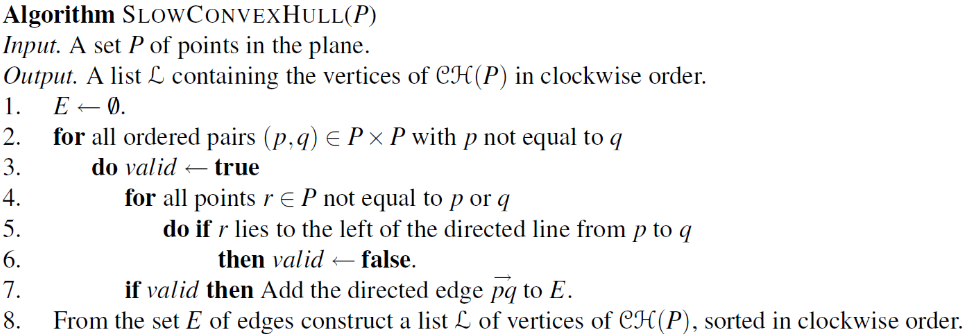
\includegraphics[width=0.9\linewidth]{afbeeldingen/slowconvexhull}
		\label{fig:slowconvexhull}
	\end{figure}
	
	De eerste lus zal $n^2$ keer lopen, gezien het voor elk paar hetgeen in de lus zal uitvoeren. In de lus zelf zal er nog eens over de punten gelopen worden om te kijken of deze allemaal rechts liggen van het gegeven punt, wat nog een $n$ keer zal lopen. De tijdscomplexiteit van dit algoritme is dus $O(n^3)$. 
	
	Naast het feit dat het algoritme helemaal niet efficiënt is, zijn er ook wat problemen in verband met de nauwkeurigheid van het berekenen of zo een punt links of rechts licht van een ander punt. Het kan zijn dat hierdoor punten fout worden bepaald terwijl ze wel links liggen van een edge. Een ander probleem is wanneer er meerdere punten op een lijn liggen, dit is dan een speciaal geval maar hier zou extra rekening mee gehouden moeten worden, het algoritme zal hier niet automatisch mee omgaan. Dit algoritme is dus duidelijk niet al te efficiënt en er zijn een paar gevallen waarbij het zelfs foute beslissingen kan maken. 
	
	
	\subsection{Incrementeel algoritme 	(Andrew's algorithm)}
	Dit algoritme zal de verzameling punten verdelen in een bovenhelft en in een onderhelft. Deze helften zullen dan in $O(n\log(n))$ volgens de x-as gesorteerd worden. Er zal dan volgens deze sortering gelopen worden om te kijken wanneer er tussen drie punten een 'rechterhoek' of een 'linkerhoek' wordt gemaakt. Als dit onduidelijk is, is hieronder een afbeelding met een voorbeeld waarom die hoeken uitmaken. 
	
	\begin{figure}[h]
		\centering
		\subfigure[]{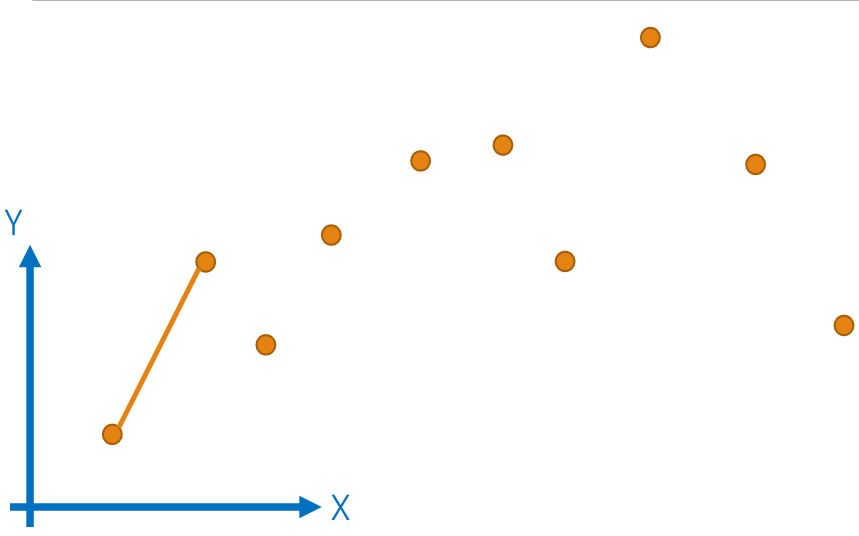
\includegraphics[width=0.24\textwidth]{afbeeldingen/first-convex}} 
		\subfigure[]{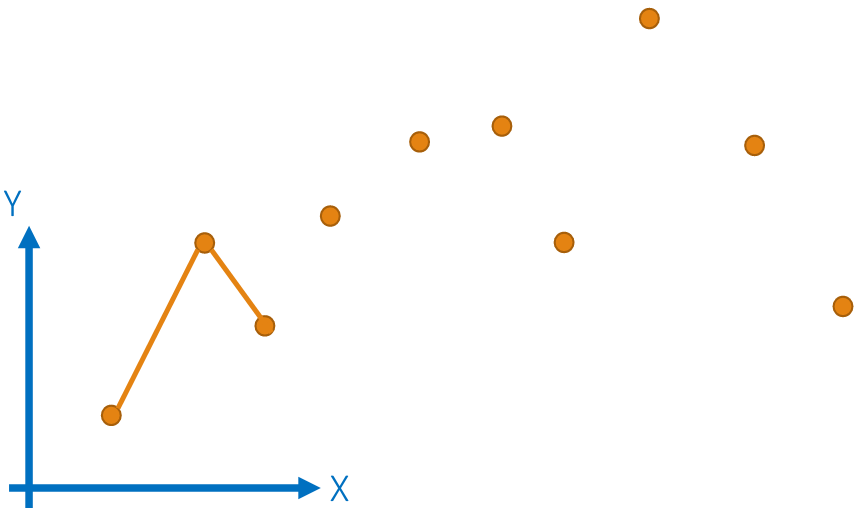
\includegraphics[width=0.24\textwidth]{afbeeldingen/second-convex}} 
		\subfigure[]{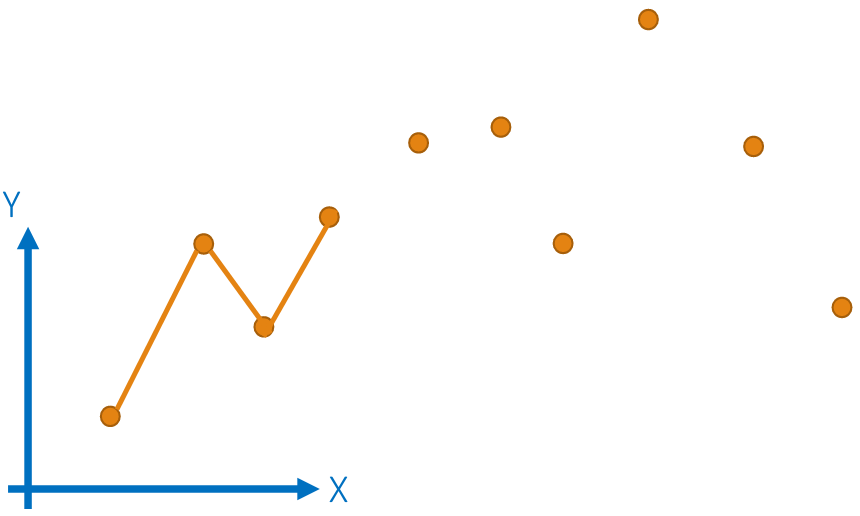
\includegraphics[width=0.24\textwidth]{afbeeldingen/third-convex}}
		\subfigure[]{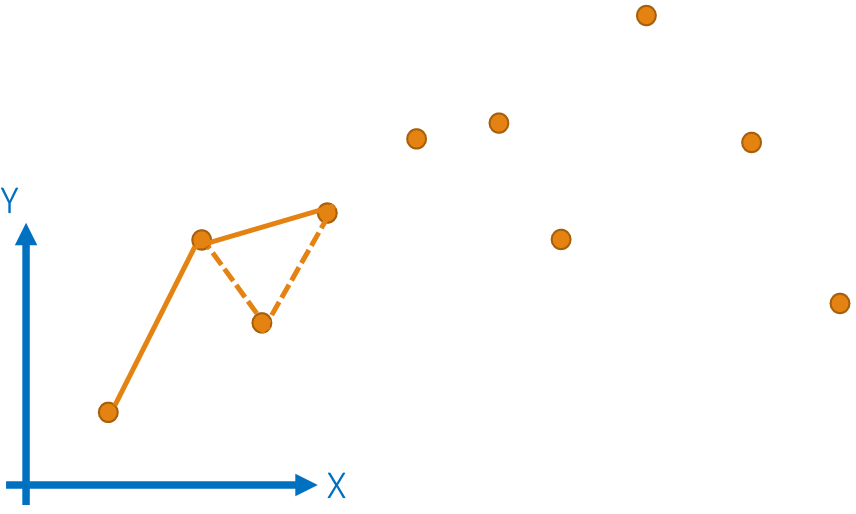
\includegraphics[width=0.24\textwidth]{afbeeldingen/fourth-convex}}
		\label{fig:incremental-example}
	\end{figure}
	Bij afbeelding c maken die punten duidelijk een linkerdraai, wat niet zou mogen voor een convex hull, dus zullen de twee edges verwijderd worden en vervangen worden door de nieuwe. Dit zal voor heel het puntenwolk verdergaan voor de bovenste helft. Voor duidelijkheid is hieronder nog de psuedocode
	\begin{figure}[h]
		\centering
		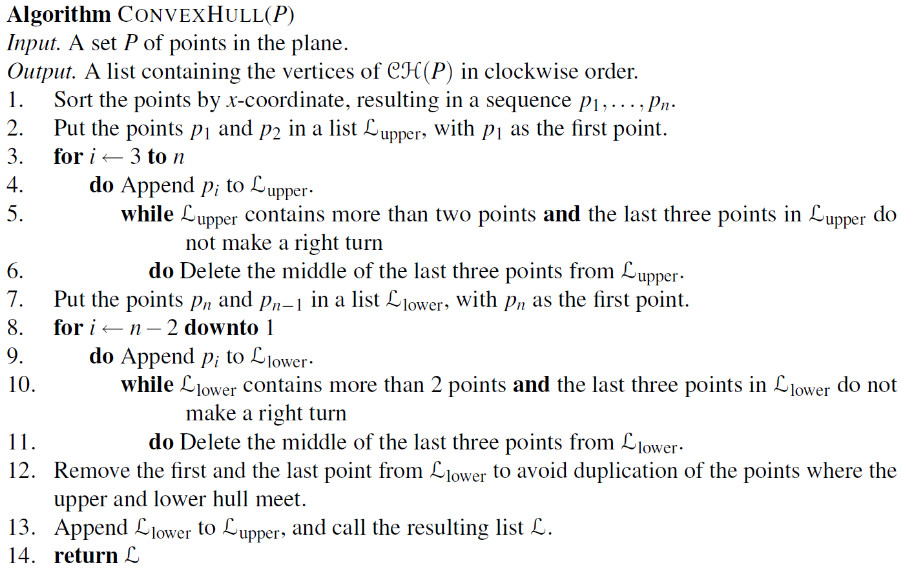
\includegraphics[width=0.9\linewidth]{afbeeldingen/convex-hull}
		\label{fig:convex-hull}
	\end{figure}

	De correctheid van het algoritme wordt bewezen d.m.v inductie: 
	\begin{itemize}
		\item Juiste bovengrens wordt berekend ${p_1, p_2}$
		\item Veronderstel dat we de juiste bovengrens berekend hebben voor ${p_1, p_2, ..., p_{i-1}}$
		\begin{itemize}
			\item $p_i$ toevoegen aan bovengrens - nieuwe bovengrens ligt boven de oude bovengrens
			\item Liggen alle punten ${p_1, p_2, ..., p_i}$ die niet behoren tot de bovengrens, beneden die bovengrens?
			\item Omwille van inductie tot $p_{i-1}$, kan enige mogelijkheid zijn dat een punt tussen $p_{i-1}$ en $p_i$ boven de bovengrens ligt, maar dit is onmogelijk, vermits we punten in gesorteerde volgorde behandelen. 
		\end{itemize}
	\end{itemize}
	Voor de tijdscomplexiteit weten we dat het sorteren van de punten $O(n\log(n))$ zal zijn terwijl voor de rest van het algoritme, we hoogstens één keer over elk punt zullen lopen, wat een tijdscomplexiteit geeft van $O(n)$. De totale tijdscomplexiteit van dit algoritme is dus \(O(n) + O(n\log(n)) = O(n\log(n))\).
	
	Ook voor dit algoritme zijn er speciale gevallen: wat als punten collineair zijn, wat met punten die hetzelfde x-coordinaat hebben en wat als er afrondingsfouten zijn in de hoeken. Dit kan allemaal opgelost worden met extra statements, maar dat geeft een lelijker algoritme. 
	
	
	\subsection{Graham's scan}
	Graham's scan zal niets aan het maken van de convex hull veranderen, maar zal het sorteren aanpassen. De punten zullen gesorteerd worden volgens poolhoek rond laagste meest linkse punt. Na het sorteren zullen de punten volgens de hoek overlopen worden om dan het verdere incrementeel algoritme toe te passen. De eerste van twee afbeeldingen bij Jarvis' march is een goede representatie van hoe de punten gesorteerd worden. 
	
	De tijdscomplexiteit is als volgt te bepalen. Het bepalen van het laagste punt is $O(n)$, het sorteren van de punten volgens punten zal $O(n\log(n))$ vragen en het overlopen zal zoals het vorige algoritme $O(n)$ vragen. De totale tijdscomplexiteit is dus $O(n\log(n))$. 
	
	
	\subsection{Jarvis's March}
	Jarvis' march zal beginnen zoals Graham's scan, beginnen met het uiterst links onderste punt en dan op poolhoeken sorteren, en zal die voor elk punt opnieuw doen. Dit wordt verduidelijkt door de onderstaande afbeeldingen; 
	
	\begin{figure}[h]
		\centering
		\subfigure[]{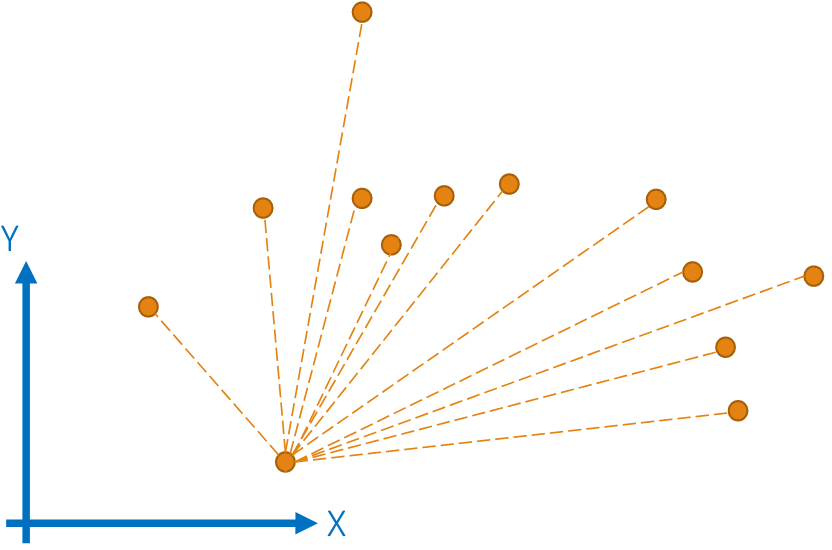
\includegraphics[width=0.45\textwidth]{afbeeldingen/first-jarvis}} 
		\subfigure[]{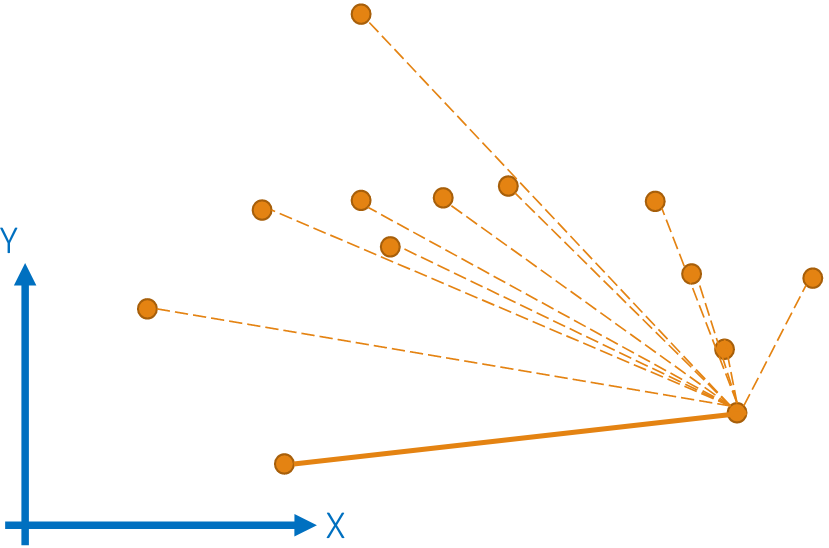
\includegraphics[width=0.45\textwidth]{afbeeldingen/second-jarvis}} 
		\label{fig:jarvis' example}
	\end{figure}

	Voor elk hoekpunt zal gekeken worden naar alle andere punten in de ruimte, hier voelen we aan dat in onze complexiteitsanalyse, we rekening zullen moeten houden met het aantal hoekpunten. Dit is het eerste algoritme waarbij we rekening houden met de output, wat resulteert in een \textit{output-afhankelijke tijdscomplexiteit}. Het aantal hoekpunten en dus het aantal elementen in de output zal in de tijdscomplexiteit $h$ zijn. Gezien we voor elk hoekpunt ongeveer alle andere punten moet overlopen, is de tijdscomplexiteit $O(n\cdot h)$.
	
	Dit algoritme zal dus bijna lineaire tijd hebben bij heel weinig hoekpunten, wat veel beter is dan graham's scan. Anderzijds kan het bijna een kwadratische tijdscomplexiteit worden als het aantal hoekpunten even groot wordt als het algemeen aantal punten. 
	
	Jarvis' march zal bij een klein aantal hoekpunten het logisch algoritme zijn terwijl graham's scan beter is voor een groter aantal. 
	
	%TODO navragen!
	

	\subsection{Verdeel-en-heers}
	Dit is een strategie die we al hebben zien terugkeren bij sorteeralgoritmes. We splitsen het probleem op, we lossen de kleinere problemen op en dan combineren we de oplossingen. De recursie stopt als de verzameling triviaal klein wordt. De tijdscomplexiteit van zo'n algoritmes is vaak $O(n\log(n))$. 
	
	Een manier is om de puntenwolk telkens willekeurig te verdelen en dan de twee convex omhullenden telkens te mergen op de meest extreme punten. Dit lijkt al heel goed, maar willekeurig kan ook heel slechte algoritmes brengen, dus is dit niet altijd het meest ideale. 
	
	Een tweede manier is om de puntenwolk telkens perfect in twee te verdelen volgens de x-coördinaten. De merge-operatie is dan telkens een bovenraaklijn en een onderraaklijn zoeken om deze te verbinden en nog steeds een convex omuhllende te verkrijgen. Deze onder- en bovenbrug is niet altijd het onderste en/of bovenste punt van een puntenwolk, hier bestaat dus een algoritme voor: 
	
	\begin{figure}[h]
		\centering
		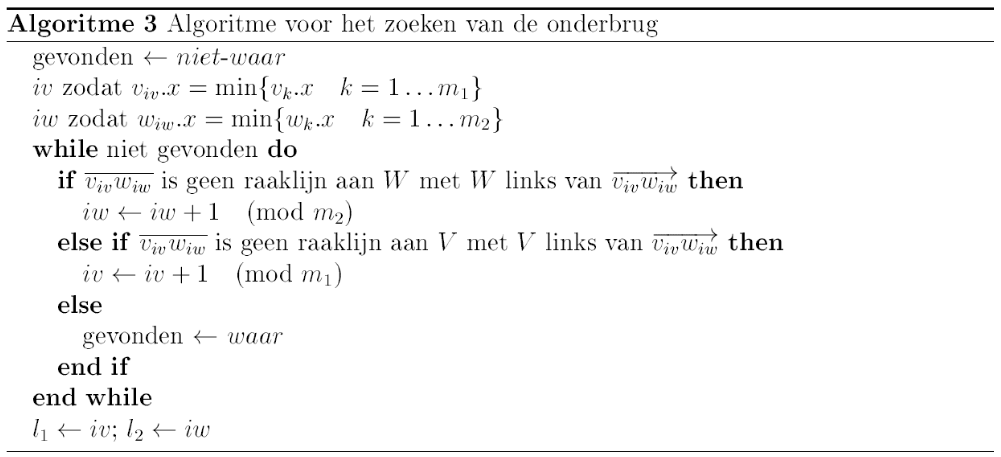
\includegraphics[width=0.9\linewidth]{afbeeldingen/verdeel-en-heers-convex}
		\label{fig:verdeel-en-heers-convex}
	\end{figure}
	%TODO verdere uitleg zoeken want hier zou mondelinge uitleg best ook bijkomen
	
	%TODO Typische examenvragen nog op te lossen
	\subsection{Typische examenvragen}
	\begin{itemize}
		\item \textbf{Leg het Graham Scan algoritme uit voor de berekening van een convex omhullende veelhoek ven een set punten:}\\
		\item \textbf{Hoe zou je Graham's Scan en Jarvis' March met elkaar vergelijken? Wat zijn sterke en zwakke punten van beide algoritmen?:}\\
		\item \textbf{Stel dat je een verzameling punten hebt, waarvan een deel punten  colineair zijn (ttz op dezelfde lijn liggen). Welke problemen zou je kunnen ontmoeten bij het Graham's Scan algoritme? Bij Jarvis' March?:}\\
		\item \textbf{Stel dat je de convex omhullende wil berekenen van een set van n lijnsegmenten. Hoe zou je dit aanpakken?:}\\
		\item \textbf{Zou je het verdeel-en-heers algoritme ook kunnen toepassen als je de verzameling punten in 4 verdeelt - bijvoorbeeld zowel via de x-mediaan als de y-mediaan? Op welke manier kan je dan 4 convex omhullende veelhoeken combineren tot 1 veelhoek?:}\\
		\item \textbf{Bij het verdeel-en-heers algoritme kan je zowel een verdeling van de x-mediaan als volgens de y-mediaan toepassen. Op alle recursieve niveau's zou je telkens een andere beslissing kunnen nemen (verdelen volgens x of y). Van welke factoren zou deze keuze kunnen afhangen?:}\\
		\item \textbf{In welke mate is algoritme *vul hier een convex omhullende algoritme in * bestand tegen kleine rekenfouten? Levert het algoritme telkens een gesloten veelhoek? Soms zelfs geen veelhoek? Een concave veelhoek? Wat zijn mogelijke oorzaken van dergelijke fouten?:}\\
	\end{itemize}


	\section{Intersecties van lijnstukken}
	In dit hoofdstuk worden algoritmes besproken om snijpunten tussen lijnstukken te vinden. 
	\subsection{Brute Force algoritme}
	Het brute force algoritme zal domweg, zoals wel verwacht, elk lijnstuk met elk ander evalueren op een snijpunt. De pseudocode ervoor is hier te vinden:
	\begin{figure}[h]
		\centering
		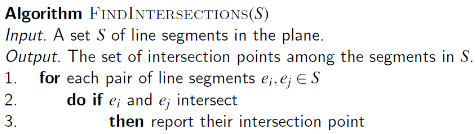
\includegraphics[width=0.8\linewidth]{afbeeldingen/find-Intersections}
		\label{fig:find-intersections}
	\end{figure}
	Het is duidelijk dat de tijdscomplexiteit van dit algoritme dus altijd $O(n^2)$ zal zijn en dat dit een \textit{input-afhankelijke} complexiteit heeft. Wanneer elk lijnstuk met elkaar snijdt kan dit geen kwaad, maar als geen enkel lijnstuke met een ander snijdt, zal je hier heel veel tijd mee verliezen. 
	
	
	\subsection{Doorlooplijn algoritme}
	%TODO stel u voor, ge weet ondertussen nog niet wat een doorlooplijn is
	Een doorlooplijn is een denkbeeldige lijn die door de dataset loopt en bijhoudt welke lijnsegmenten actief zijn en dus potentieel elkaar kunnen snijden. Als twee lijnsegemnten op die lijn zitten kan het zijn dat ze elkaar snijden, als ze niet op een moment gelijktijdig op de lijn zitten, is er geen kans dat ze elkaar snijden en moeten ze dus niet geëvalueerd worden op snijpunten. Als eerste zullen de punten dus gesorteerd moeten worden op de y-as volgens de begin- en eindpunten van de lijnsegmenten. Deze zouden dan terechtkomen in een event queue om deze af te lopen en bij elk punt een actie te ondernemen. Bij een startpunt worden alle actieve lijnsegemten geëvalueerd met het nieuwe toegevoegde lijnsegmenten om snijpunten te zoeken. Zo wordt een deel van de lijnsegmenten gefilterd en is het geen bruteforce. De datastructuur voor de doorlooplijn zou in dit geval gewoon een lijst kunnen zijn aangezien deze niet gesorteerd hoeven te zijn. 
	
	De worst case van dit algoritme is wanneer er allemaal lijnstukken parallel verticaal naast elkaar liggen. Dan wordt elk lijnstuk met elkaar vergeleken ondanks dat we een doorlooplijn gebruiken en is het even onefficiënt als een brute force algoritme. 
		
	\subsection{Doorlooplijn++}
	In de verbeterde doorlooplijn zullen we niet naar alle actieve lijnstukken kijken op de lijn, maar enkel naar de buren van het toegevoegde lijnstuk. Nu zal er dus wel een datastructuur nodig zijn om deze sortering bij te houden, dit zal het beste gaan met een gebalanceerde zoekboom. Er zijn verschillende soorten 'events' in dit algoritme, je kan van elk een voorbeeld zien in de onderstaande afbeelding.  
	
	\begin{figure}[h]
		\centering
		\subfigure[]{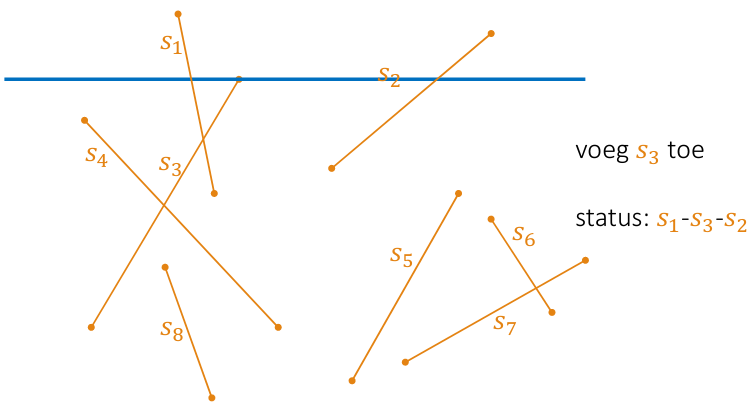
\includegraphics[width=0.24\textwidth]{afbeeldingen/first-doorlooplijn}} 
		\subfigure[]{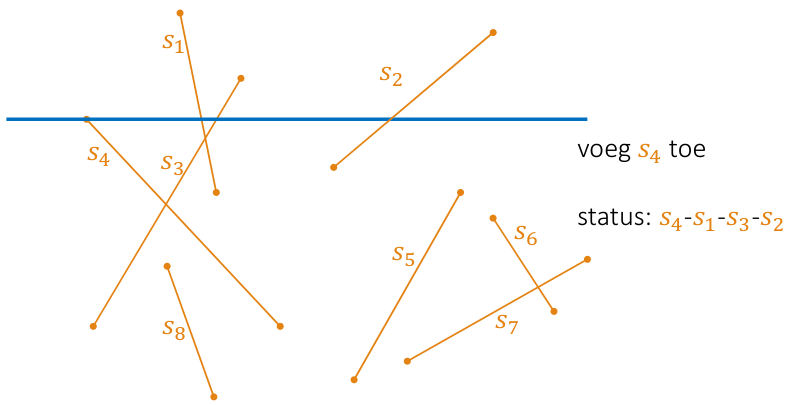
\includegraphics[width=0.24\textwidth]{afbeeldingen/second-doorlooplijn}} 
		\subfigure[]{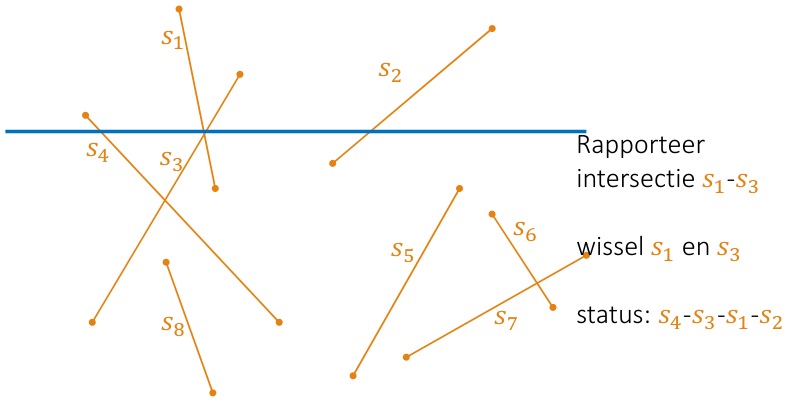
\includegraphics[width=0.24\textwidth]{afbeeldingen/third-doorlooplijn}}
		\subfigure[]{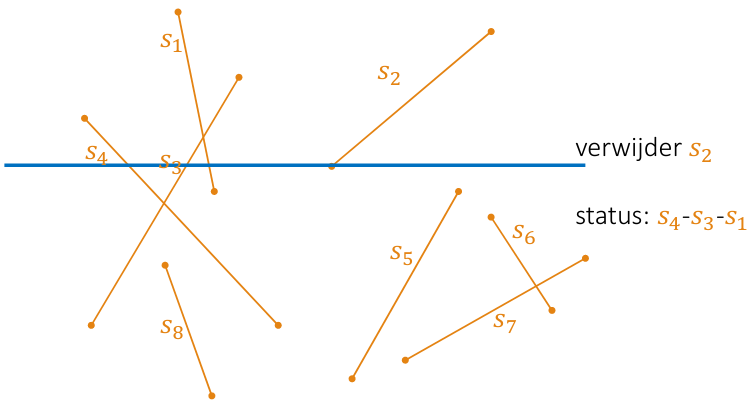
\includegraphics[width=0.24\textwidth]{afbeeldingen/fourth-doorlooplijn}}
		\label{fig:sweepline-example}
	\end{figure}

	De event queue zal in dit geval ook een gebalanceerde zoekboom zijn, het is geen priority queue aangezien er niets is dat een 'prioriteit' heeft.
	\begin{description}
		\item[Start event:] Een start event is wanneer een nieuw lijnstuk actief wordt op de doorlooplijn, in dat geval zal het nieuwe lijnstuk vergeleken worden met zijn buren op snijpunten. Als er snijpunten worden gevonden, worden deze toegevoegd aan de event queue. 
		\item[intersectoin event:] Bij een snijpunt zal het algoritme de volgorde van de lijnstukken op de status queue verwisselen en deze lijnstukken zullen dan met hun nieuwe buren vergeleken worden voor nieuwe snijpunten. 
		\item[End event:] Het einde van een lijnstuk betekent dat dit lijnstuk van de status queue gehaald moet worden en dat er moet gekeken worden of de nieuwe buren elkaar snijden. 
	\end{description}

	De pseudocode is hieronder te vinden: 
	
	\begin{figure}[h]
		\centering
		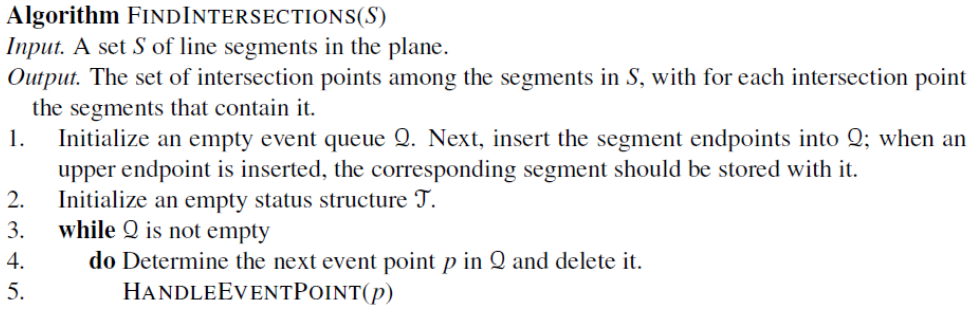
\includegraphics[width=0.9\linewidth]{afbeeldingen/find-intersections++}
		\label{fig:find-intersections++}
	\end{figure}
	
	De correctheid van dit algoritme wordt als volgt bewezen: Indien twee lijnsegmenten elkaar snijden, moet er ergens een event zijn boven het intersectiepunt, waar beide lijnsegmenten elkaars buren worden.\\
	Indien de doorlooplijn zich net boven een intersectiepunt p bevindt, zijn $s_i$ en $s_j$ aangrenzend (en worden dus getest op intersectie).\\
	Initieel is de status leeg, er moet dus ergens een event zijn dat $s_i$ en $s_j$ aangrenzend maakt.
	
	Elk event is begrensd door een tijdscomplexiteit van $O(\log(n))$. De lus zal 2n + k keer uitgevoerd worden, met $n$ het aantal cirkels en $k$ het aantal snijpunten. De lus zal dus  $O(n + k)$ overlopen worden, wat een totaal geeft van $O((n+k)\log(n))$. Qua geheugen zal de status vast zijn door het maximaal aantal elementen dat er op de lijn tevoorschijn kan komen, wat dus $O(n)$ is. De event queue zal begrensd zijn door $2n + k$ events, wat in het ergste geval kan uitkomen op $O(n^2)$. 
	
	Een speciaal geval kan twee punten zijn die dezelfde y-waarde hebben, dan kan de event queue het niet juist sorteren. Dit kan opgelost worden door de doorlooplijn zogezegd wat schijner te laten lopen. Een ander probleem is het samenvallen van events (het einde van een lijnstuk is gelijk aan het begin van een ander lijnstuk.) Hier moeten dan tijdens het implementeren bepaalde keuzes gemaakt worden, maar dit kan ook opgelost worden. %TODO moet hier nog iets bij? 


	\subsection{Doubly-connected edge list}
	Een DCEL is een manier om een oppervlak met lijnen in een datastructuur te steken en zo gemakkelijk over de datastructuur kunnen verplaatsen. Eerst volgen wat termen die belangrijk zijn om te kunnen praten over deze DCEL. 
	
	\begin{figure}[H]
		\centering
		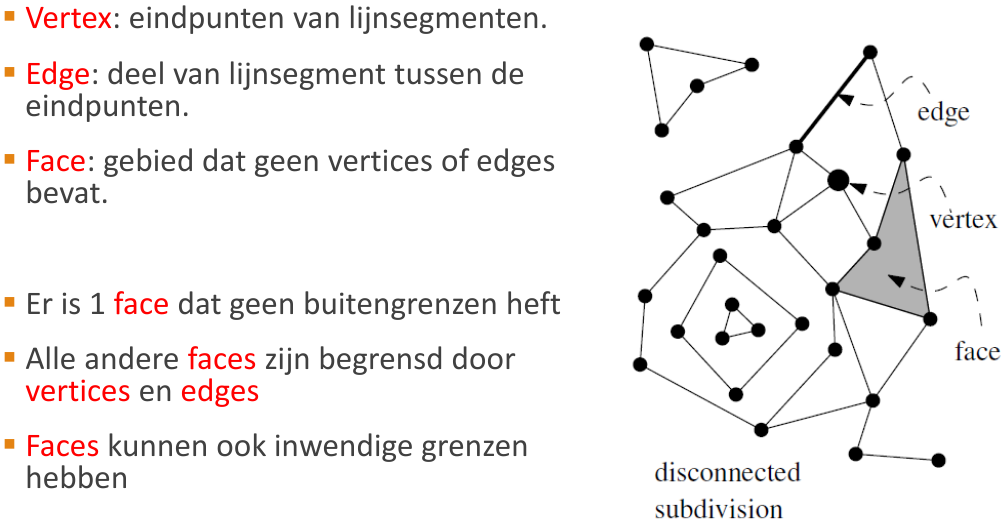
\includegraphics[width=0.8\linewidth]{afbeeldingen/DCEL-termen}
		\label{fig:dcel-termen}
	\end{figure}

	Het centrale idee is dat elke edge uit bovenstaande afbeelding kan gemaakt worden uit 2 'half-edges'. Deze half edges hebben elk een oorsprong-vertex, een twin (de andere half edge), een incidentface (face aan de linkerkant van de half-edge), een next en een prev. Elke vertex bestaat uit coördinaten en een incidentEdge (de edge startende in de vertex). 
	
	Met deze datastructuur kunnen we gemakkelijker de overlay van twee vlakverdelingen bepalen. Dit is eignelijk aanvankelijk het construeren van een DCEL uit twee DCEL's, wat door een doorloopalgoritme zal gebeuren. Ook hier werken we met events: 
	\begin{itemize}
		\item Een vertex van S1
		\item Een vertex van S2
		\item Een intersectiepunt van een edge van S1 met een edge van S2. 
		\begin{figure}[H]
			\centering
			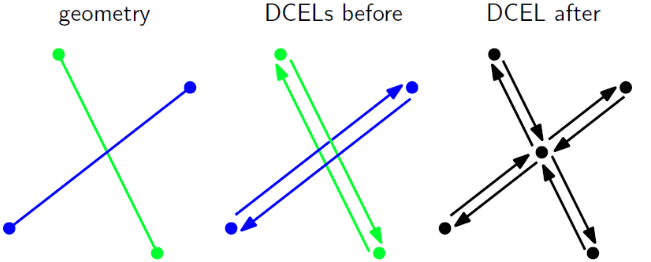
\includegraphics[width=0.7\linewidth]{afbeeldingen/intersection-DCEL}
			\label{fig:intersection-dcel}
		\end{figure}
		\item De edge van S1 snijdt met een vertex van S2 (of omgekeerd)
		\begin{figure}[H]
			\centering
			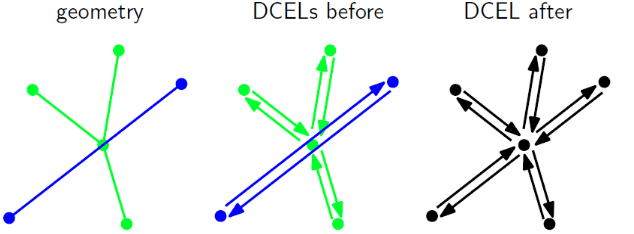
\includegraphics[width=0.7\linewidth]{afbeeldingen/DCEL-vertex&edge}
			\label{fig:dcel-vertexedge}
		\end{figure}
		\item Samenvallende vertices van S1 en S2
		\begin{figure}[H]
			\centering
			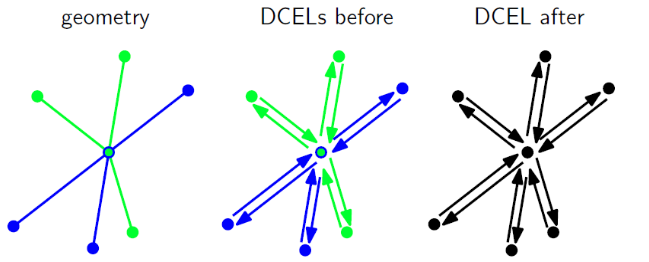
\includegraphics[width=0.7\linewidth]{afbeeldingen/DCEL-vertices}
			\label{fig:dcel-vertices}
		\end{figure}
	\end{itemize}

	Om de faces te bepalen, zal de nieuwe DCEL overlopen moeten worden om alle loops te detecteren en de inwendige en uitwendige grenzen te bepalen. Een face moet dan geconstrueerd worden voor elke uitwendige grens (+ het buitengebied). Van de inwendige grenzen kunnen we het meest links punt bepalen (van de vorm) en zodra een andere edge is gevonden, wordt deze vorm overlopen. Dit is dan de vorm waarbinnen de aanvankelijke vorm ligt. Dan kan een structuur zoals hieronder gemaakt worden. Deze indelingen zijn gemakkelijk om booleaanse opdrachten te gebruiken op veelhoeken.
	
	\begin{figure}[H]
		\centering
		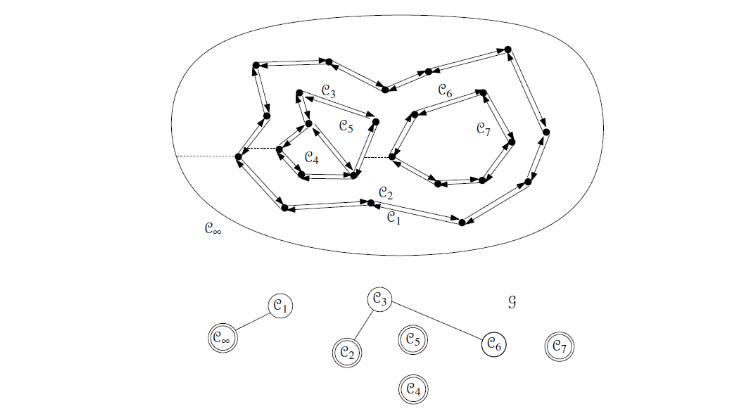
\includegraphics[width=0.7\linewidth]{afbeeldingen/DCEL-faces}
		\label{fig:dcel-faces}
	\end{figure}
	
	Voor de tijdscomplexiteit is de volgende afbeelding het bewijs (cuz ja, ik ben effe lui):
	
	\begin{figure}[H]
		\centering
		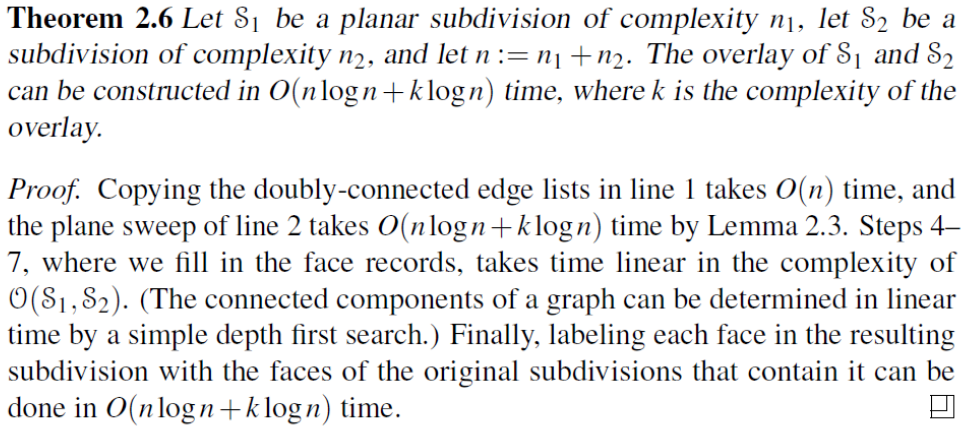
\includegraphics[width=0.7\linewidth]{afbeeldingen/DCEL-bewijs}
		\label{fig:dcel-bewijs}
	\end{figure}
	
	
	\subsection{Typische examenvragen}
	\begin{itemize}
		\item \textbf{Wat is de algemene idee van sweep-line algoritmen?:}\\
		\item \textbf{Beschrijf het algoritme om alle intersectiepunten in een verzameling lijnstukken te vinden. Bespreek ook de tijdscomplexiteit:}\\
		\item \textbf{Bespreek de Double-Connected-Edge-List als datatstructuur. Wat zijn voor- en nadelen van deze datastructuur?:}\\
		\item \textbf{Bespreek welke operaties er precies moeten gebeuren bij de afhandeling van <event van type X> bij het berekenen van de overlay van 2 vlakindelingen:}\\
	\end{itemize}
	
	
	\section{Triangulaties van veelhoeken}
	Dit deel begint met een klein voorbeeld als context. Stel dat je in een museum werkt en moet besluiten waar de bewakers 's nachts zullen staan. Je wilt natuurlijk zo min mogelijk (stilstaande) bewakers voor de ruimte die je moet bewaken. Dit wordt het \textit{Museumprobleem} genoemd. Bij deze probleemstelling komen dan ook de vraag: Wat is het minimaal aantal bewakers dat nodig is voor een n-hoek? 
	
	\subsection{Typische examenvragen}
	\begin{itemize}
		\item \textbf{Bewijs dat een oplossing voor het “museumprobleem” of “art gallery problem” voor een (eenvoudige) veelhoek met n hoeken een bovengrens heeft gelijk aan  n/3 (naar beneden afgerond) bewakers:}\\
		\item \textbf{Stel dat we een klasse (eenvoudige) veelhoeken hebben, met als eigenschap dat ze d.m.v. niet-snijdende diagonalen in de veelhoek steeds kunnen opgesplitst worden in een verzameling convexe vierhoeken. Welke uitspraken kan je doen i.v.m. het “museumprobleem” of “art gallery problem” voor deze klasse van veelhoeken?:}\\
		\item \textbf{Bewijs dat elke eenvoudige veelhoek met n hoekpunten kan getrianguleerd worden in n-2 driehoeken. Geef duidelijk alle stappen in de redenering:}\\
		\item \textbf{Op welke manier kunnen we een veelhoek splitsen in een aantal monotone veelhoeken?:}\\
		\item \textbf{In het globale algoritme om een veelhoek te trianguleren splitsen we eerst de veelhoek op in y-monotone veelhoeken. Maakt het een verschil voor de finale triangulatie als we zouden splitsen in x-monotone driehoeken?:}\\
	\end{itemize}
	
	
	\section{Lineaire programming \& gerandomiseerde algoritmen}
	
	
	
	\section{Orthogonal Range searching, Kd-bomen}
	\subsection{Typische examenvragen}
	\begin{itemize}
		\item \textbf{Wat is een kd-boom? Leg uit:}\\
		\item \textbf{Wat is de tijdscomplexiteit voor het opzoeken van alle punten binnen een (gegeven) 2D-interval in een tweedimensionale kd-boom?:}\\
		\item \textbf{Leg de idee uit van Range Trees:}\\
	\end{itemize}
	
	
	\section{Puntlocatie}
	\subsection{Typische examenvragen}
	\begin{itemize}
		\item \textbf{Leg de pincipes uit van een trapezium-map:}\\
		\item \textbf{Leg het algoritme uit om een lijnsegment toe te voegen aan een bestaande trapezium-map:}\\
		\item \textbf{Op welke manieren kunnen we nagaan of een punt behoort tot het inwendige van een veelhoek?:}\\
	\end{itemize}
	
	
	\section{Voronoi Diagramma's}
	\subsection{Typische examenvragen}
	\begin{itemize}
		\item \textbf{Wat is het verband tussen het Voronoidiagramma van een verzameling punten, en de Delaunay triangulatie?:}\\
		\item \textbf{Leg het sweep-line algoritme van Fortune uit om een Voronoidiagramma te construeren:}\\
		\item \textbf{Bewijs eigenschap X van Voronoi-diagramma's. Welk belang heeft deze eigenschap voor de algoritmische constructie van Voronoi-diagramma's?:}\\
		\item \textbf{De Voronoi-veelhoek behorend bij een punt p dat behoort tot S is begrensd als en slechts als p behoort tot het inwendige van de convex omhullende van S. Bewijs deze eigenschap. Waar wordt deze eigenschap gebruikt, of waarom is ze nuttig?:}\\
		\item \textbf{Hoe bewijs je dat een Voronoi-diagram van een verzameling van N sites maximaal 2N-5 Voronoi-punten en maximaal 3N-6 Voronoi-zijden bezit? Waarom is het belangrijk dat het aantal Voronoi-zijden (slechts) O(N) is? Geef minstens één voorbeeld van het nut van deze eigenschap:}\\
		\item \textbf{(Gegeven een tekening met een aantal punten als Voronoi-sites en een positie van de doorlooplijn). Schets op bijhorende tekening het golffront voor de positie die de doorlooplijn reeds bereikt heeft, teken eveneens de Voronoi-punten en Voronoi-zijden die het algoritme van Fortune reeds bepaald heeft. Schrijf eventueel commentaar bij je tekening om één en ander te verduidelijken:}\\
		\item \textbf{Geef een voorbeeld waarbij de parabool behorende bij een Voronoi-site méér dan 1 segment bijdraagt aan het golffront (algoritme van Fortune):}\\
		\item \textbf{Geef een voorbeeld waarbij voor 6 Voronoi-sites, elk van de 6 sites door de doorlooplijn behandeld worden, vooraleer er een cirkel-event plaatsvindt. De sites moeten algemeen van aard zijn, ttz geen 3 sites op een lijn of 4 sites op een cirkel:}\\
	\end{itemize}
	
	
	\section{Delaunay Triangulatie}
	\subsection{Typische examenvragen}
	\begin{itemize}
		\item \textbf{Leg het verband uit tussen het Voronoi-diagramma van een puntenset en de Delaunay triangulatie van diezelfde puntenset:}\\
		\item \textbf{Op welke manier kan de Delaunay-triangulatie van een puntenset geconstrueerd worden?:}\\
		\item \textbf{Leg de equivalentie uit tussen de "cirkeleigenschappen" in zowel het Voronoi-diagramma als de Delaunay-triangulatie:}\\
		\item \textbf{Gegeven een set punten met bijhorende triangulatie. Is de getekende triangulatie een Delaunay-triangulatie? Waarom wel? Waarom niet? Welke eigenschappen kan je gebruiken om dit vast te stellen?:}\\
		\item \textbf{In een getekende Delaunay-triangulatie wordt een punt toegevoegd. Schets de resulterende Delaunay-tiangulatie:}\\
	\end{itemize}
	%Opmerking: vragen waarbij gevraagd wordt handmatig na te gaan of bepaalde eigenschappen gelden in een getekende Delaunay-triangulatie of Voronoi-diagramma zullen natuurlijk geen "milimeter-werk" zijn om iedereen op stang te jagen. Vaak zou je de cirkeleigenschappen met het blote oog moeten kunnen zien of gemakkelijk moeten kunnen afleiden met een eenvoudige construtie met een meetlat of passer ...
	
	
	\section{Béziercurven}
	\subsection{Typische examenvragen}
	\begin{itemize}
		\item \textbf{Gegeven een curve met enkele controlepunten met bijhorende curve: is dit (vermoedelijk) een Béziercurve? Waarom wel, waarom niet? Welke eigenschappen gebruik je om dit te achterhalen?:}\\
		\item \textbf{Gegeven enkele controlepunten: schets zo goed mogelijk (gebruik makende van eigenschappen van Béziercurven) de resulterende Bézier-curve:}\\
		\item \textbf{Wat zijn de belangrijkste eigenschappen van Béziercurven?:}\\
		\item \textbf{Leg uit: graadverhoging in Bézier-curven:}\\
		\item \textbf{Leg uit: Splitsing van Béziercurven:}\\
		\item \textbf{Leg uit hoe bij samengestelde Béziercurven C1- of C2-continuïteit voor de samengestelde curve bekomen wordt. Illustreer dit ook grafisch:}\\
		\item \textbf{Leg de ‘variatie-verminderingseigenschap’ van Bézier-curven uit. Waarom is deze belangrijk bij het ontwerp van curven?:}\\
		\item \textbf{Hoe vertaalt eigenschap X van Bernstein-veeltermen zich naar het gedrag van Bézier-curven?:}\\
	\end{itemize}
	
	
	\section{Binairy Space partitions}
	%The spiderman one
	\subsection{Typische examenvragen}
	\begin{itemize}
		\item \textbf{Wat is een Binary Space Partioning boom?:}\\
		\item \textbf{Bewijs dat een lage densiteits BSP boom O(n/k) bladknopen heeft:}\\
		\item \textbf{Wat is de bedoeling van de krimp-stap bij het opbouwen van een lage densiteits BSP boom?:}\\
		\item \textbf{Wat is het verband tussen een kd-boom en een BSP-boom?:}\\
		\item \textbf{Wat is de definitie van de dichtheid (density) van een set van objecten? Welk nut heeft de definitie van densiteit bij het opbouwen van een spatiale binaire zoekstructuur?:}\\
	\end{itemize}
	
	
	\section{Motion planning \& Visibility graphs}
\end{document}